\section{Pourquoi se conformer à un standard ? }
    \subsection{Un langage recommandé pour l’édition scientifique numérique}

Les corpus encodés en \TEI sont de plus en plus nombreux dans les projets de recherche en humanités numériques. La \TEI permet de préconiser des standards d'encodage au format \XML. Ces préconisations sont documentées dans les \textit{guidelines} disponibles en ligne et permettent d'assurer l'interopérabilité des données encodées en \XML pour l'édition scientifique numérique, en privilégiant un encodage sémantique afin de décrire les documents. Ce standard permet de s'adapter à un grand nombre de documents, nativement numériques ou transpositions de sources matérielles, et offre donc de nombreuses possibilités d'encodage et un niveau de personnalisation élevé, ce qui explique son utilisation de plus en plus majoritaire dans les projets d'édition scientifique numérique.

\begin{quote}
    La TEI met l’accent sur ce qui est partagé par tous les types de documents, qu’ils soient représentés physiquement sous une forme numérique sur un disque ou une carte mémoire, sous une forme imprimée comme un livre ou un journal, sous une forme écrite comme un manuscrit ou un codex, ou sous une forme inscrite dans la pierre ou sur une tablette de cire. Cette continuité facilite la migration du texte depuis des manifestations plus anciennes, comme l’imprimé ou le manuscrit, vers d’autres plus récentes comme le disque ou l’écran. \footnote{\cite{burnard_tei_2015}}
\end{quote}

En s'adaptant à tous types de documents, la \TEI représente un format de données idéal pour le projet \COREL : les textes de lois étant produits selon une architecture définie et régulière, ils se prêtent particulièrement bien à un encodage sémantique, qui permet de mettre en avant les éléments structurants des textes. De plus, la \TEI offre un vaste choix de balises, ce qui permet aux chercheurs de pouvoir enrichir leurs sources, conformément aux objectifs du projet. Encoder les documents en \TEI garantit à la fois un encodage régulier et cohérent grâce à sa documentation, flexible et bien adapté aux sources grâce aux nombreuses possibilités d'encodage. Le passage à des documents encodés en \TEI, en plus de contribuer à l'interopérabilité des données de la recherche, assure aux chercheurs une indépendance dans les choix éditoriaux, contrairement au schéma figé du projet \LSC utilisé jusqu'à présent. Malgré la richesse de la \TEI, il est possible que l'utilisation de certains éléments ne correspondent pas entièrement aux spécificités d'un texte. Toutefois, ce cas de figure est également prévu par la \TEI. Il est en effet possible d'étendre le standard en modifiant le schéma d'encodage dans l'\ODD. Deux types de modifications de la \TEI sont alors possibles : des modifications dites \TEI \textit{conformant}, qui respectent les règles de la \TEI, ou bien des modifications qui outrepassent ces règles, bien que ces dernières ne soient pas conseillées. Que la \TEI soit étendue ou non, il est essentiel d'avoir un projet bien documenté, qui permette à d'autres utilisateurs de la \TEI de comprendre comment les données ont été structurées et quels choix d'encodage ont été faits. 

\subsection{Interopérabilité et documentation en ligne}

La \TEI a été créée en 1987 pour promouvoir un standard d'encodage des données en humanités numériques et ainsi permettre l'interopérabilité des ressources en ligne. En effet, le numérique apporte un foisonnement de données et de formats divers et souvent incompatibles entre eux, qui rendent l'échange des données difficile, voire impossible. Établir un standard de la diffusion des données en \textit{open access} afin de garantir leur accessibilité devient un enjeu majeur corrélé à l'apparition du web et à l'essor des formats propriétaires au profit des entreprises privées. Bien que les principes de science ouverte continuent de se développer aujourd'hui, il est primordial de maintenir la conformité à des standards afin de produire des données \fair et pérennes. 

Les principes \fair des données sont l'un des enjeux du projet \COREL. En effet, les chercheurs ont été sensibilisés à l'importance de l'ouverture des données via le projet \LSC, qui présente de nombreuses contraintes résultant du manque d'\textit{open access}. Les données \XML n'étant pas libre d'accès ni interopérables, et le site internet propriétaire ne répondant plus aux besoins d'évolution du projet, contribuer à la science ouverte et faciliter l'accès aux sources (les textes de lois mais aussi leur transposition en sources numériques) est primordial afin d'enrichir les sources du droit chinois dans le domaine du numérique. 

L'encodage des données en \TEI permet de produire des données interopérables et réutilisables par la communauté de chercheurs en sciences humaines, selon les recommandations du \w. C'est également un avantage pour l'équipe du projet, qui peut se référer aux \textit{guidelines} et accéder à une documentation claire et fournie, ce qui permet de faire des choix d'encodage adaptés et d'obtenir des documents \TEI valides. Cela permet aussi de se nourrir d'autres projets de recherche qui utilisent la \TEI et de pouvoir accéder à des outils de publication de données comme \tp. En effet, de nombreux exemples de données encodées en \TEI et publiées avec \tp sont disponibles en ligne. Dans le cadre du projet \COREL, deux exemples ont notamment été étudiés : le projet \disco de l'INRIA, qui présente des éditions scientifiques numériques de correspondances et le projet \cordel de l'Université de Genève. Ces deux exemples permettent d'illustrer l'adaptabilité du langage \TEI, qui permet d'encoder des documents très différents : des correspondances, de la littérature de colportage ou, dans le cas du projet \COREL, des textes de lois. 

 \section{La transformation en XML-TEI}
    \subsection{Une transformation adaptée aux besoins du projet}
    
En plus de pouvoir s'appuyer sur des exemples de projets de recherche, encoder les documents du corpus en \TEI a permis d'établir un schéma d'encodage stable. En effet, les balises \TEI sont documentées dans les \textit{guidelines} et ont une utilisation prédéfinie, ce qui permet d'assurer la régularité de l'encodage au fur et à mesure du projet. Contrairement au schéma \LSC qui proposait une petite quantité de balises dont l'usage initial à été détourné au fil du temps, comme par exemple les balises \texttt{<content/>}, un encodage en \TEI diminue le risque de mésusage des balises grâce à sa documentation. De plus, l'encodage du projet a pu s'écarter d'un schéma pensé pour l'affichage du texte afin d'adopter l'orientation sémantique de la \TEI. À court termes, cette pratique d'encodage offre une meilleure compréhension et structuration des documents, qui n'est plus liée à son affichage \HTML. À long termes, un encodage sémantique permet de produire un jeu de données qui pourra être réutilisé par les chercheurs. 

Il est pertinent de considérer les données comme un matériau à partir duquel le projet produit des livrables : si certains chercheurs en histoire du droit chinois consulteront le produit fini que sera le site web du projet, d'autres, initiés aux humanités numériques, pourront également consulter les données \TEI et les prendre comme support pour leurs propres recherches. Dissocier les données des livrables permet aussi d'enrichir les données de la recherche, puisque le projet \LSC notamment n'offre pas de données en libre-accès mais simplement les résultats produits à partir de ces données. Cette pratique d'un encodage sémantique, interopérable vient donc répondre à l'une des problématiques principales du projet au début du stage : la réutilisation de données produites pour un projet spécifique, qui ne respectent pas les principes \fair des données puisqu'elles ne sont pas disponibles en ligne librement (l'accès au site web \LSC est possible, mais les données ne sont pas mises à la disposition des chercheurs), non-interopérables car malgré le format d'encodage \XML, le schéma est entièrement personnalisé et non-documenté, ce qui aboutit enfin à des données qui peuvent difficilement être réutilisées. Le projet \COREL, en transformant ces données en \TEI, contribue ainsi à la science ouverte et à l'enrichissement des données de la recherche, tout en bénéficiant d'un encodage mieux adapté aux besoins du projet. 

\subsection{La transformation XSLT}

Le projet \cordel est l'un des exemples sur lequel le projet \COREL prend appui. Les données des deux projets présentent en effet des similarités. Issues de l'\OCR, les données ont d'abord été encodées en \XML. Pour le projet \COREL, cet encodage provient d'un projet antérieur, tandis que pour le projet \cordel, les données de l'\OCR ont été encodées automatiquement par \textit{Transkribus}. À l'instar de l'Université de Genève, les données des codes légaux chinois ont ensuite été transformées via le langage \XSLT en documents \TEI valides. 

Le langage \XSLT est un langage \XML conçu pour transformer des documents \XML en documents \XML, \HTML ou \LaTeX. Un document \XML en entrée passe par un processeur \XSLT avec des instructions \XSL rédigées dans une feuille de style.

\begin{figure}
    \centering
    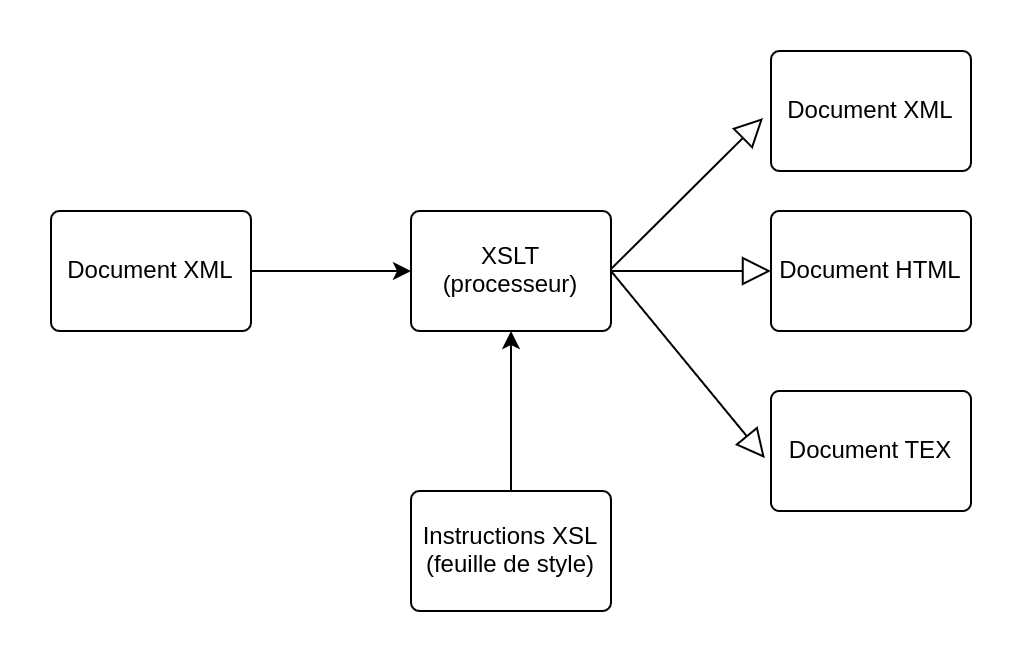
\includegraphics[width=\textwidth]{images/xslt.png}
    \caption{Modélisation de la transformation \XSLT}
\end{figure}

Les données du projet \LSC conservent la structure générale des codes légaux chinois. Cela facilite la transformation \XSLT qui maintient cette structure en chapitres, sections et lois en sélectionnant uniquement les éléments structurants. Toutefois, l'une des difficultés de cette transformation, malgré la structure rigoureuse des textes chinois, découle de la modification des pratiques d'encodage dans le temps. En effet, puisque certaines balises sont utilisées selon des usages différents d'un document à l'autre, il est nécessaire de penser les règles de transformation avec de nombreuses exceptions. Ces contraintes ont donné lieu, dans un premier temps, à un code verbeux à l'intérieur duquel de nombreuses conditions \texttt{<xsl:if/>} et \texttt{<xsl:when/>} étaient imbriquées. Le code, en plus d'être difficile à lire, risquait de plus d'aboutir à des erreurs sur certaines de ces exceptions, erreurs difficilement repérables puisque je ne suis pas en mesure de lire les documents chinois. 

Dans ces circonstances, il est essentiel d'écrire un code qui soit le plus clair et simple possible, pour aboutir à un risque d'erreur faible. Les nombreuses conditions imbriquées les unes dans les autres, en plus d'être compliquées à lire et de présenter un risque d'erreur important si l'une des conditions n'est pas remplie, peut également complexifier les chemins \xpath à renseigner dans les règles de transformation puisque le \xpath tient compte de ces imbrications : il faut ainsi toujours tenir compte du noeud courant spécifié dans la règle parente. 

\begin{minted}{xslt}
     <xsl:for-each select="./li">
        <div type="substatute">
            <xsl:attribute name="n">
                <xsl:value-of select="./@id"/>
            </xsl:attribute>
            <pb/>
            <xsl:for-each select="./content[@lang='ch']">
                <p>
                    <xsl:apply-templates/>
                </p>
            </xsl:for-each>
        </div>
    </xsl:for-each>
\end{minted}

Dans cet exemple simple d'une règle pour reproduire les \li dans un élément \texttt{<div/>}, trois chemins \xpath sont nécessaires : le premier sélectionne toutes les balises \texttt{<li/>} du document \XML, et les deux autres sélectionnent des éléments ou attributs à partir du noeud courant, c'est-à-dire contenus à l'intérieur de la balise \texttt{<li/>}. De plus, les \li sont des articles additionnels, qui sont donc contenus dans des éléments parents (les \lu). Il est ainsi possible d'observer qu'une règle simple, sans conditions particulières, requiert déjà une attention accrue portée au \xpath. Utiliser des règles imbriquées trop profondément les unes dans les autres pour transformer des documents que je suis incapable de lire n'était donc pas la solution idéale pour traiter les données. Écrire des règles complexes afin de prendre en compte les spécificités de chaque document, que leur lecture soit possible ou non, n'est d'ailleurs pas une solution adaptée au traitement d'un grand nombre de données. En effet, un code trop complexe et difficile à corriger risque de produire des erreurs qui ne seront pas repérées à la vérification, car il n'est pas envisageable de relire tous les documents un à un. 

Toutefois, le corpus étant composé d'un petit nombre de documents, une granularité fine de la feuille de style est envisageable, c'est pourquoi les règles de transformation ont été divisées en plusieurs éléments \texttt{<xsl:template/>} : un template pour rédiger le \texttt{<teiHeader/>} commun à tout le corpus puis un template pour chaque document du corpus. 

\begin{minted}{xslt}
    <!-- Nouveau template pour le code de 1740 -->
    <xsl:template match="/code[@id='DQLL1740']/document">
    ...
    </xsl:template>

    <!-- Nouveau template pour le code de 1646 -->
    <xsl:template match="/code[@id='code1646']/document">
    ...
    </xsl:template>
\end{minted}
Dans les sources numériques du projet \LSC, chaque document a un identifiant unique, ce qui permet de faire un template par code légal, tout en ayant des templates généraux comme pour le \texttt{<teiHeader/>}. Rédiger un template pour chaque document peut sembler redondant puisque la structure globale des textes de lois reste la même (chaque template présente une règle sur les chapitres, les sections, les \lu et les \li). Toutefois, des variations dans l'encodage sont difficile à prendre en compte dans un seul template : notamment l'usage de la balise \texttt{<content/>} comme vu précédemment, mais aussi des variations entre les codes légaux et les compilations. Le \huidian par exemple présente du contenu supplémentaire, encodé dans des balises \texttt{<part/>}, qui contiennent des listes de lois. Pour prendre en compte ces exceptions, l'utilisation de plusieurs templates permet de rendre le code plus lisible et moins verbeux. De plus, les données \LSC continuant d'être enrichies en parallèle du projet \COREL, la feuille de style n'est pas un outil à usage unique et est amenée à être modifiée par d'autres, ce qui renforce l'intérêt de produire un code clair et compréhensible. 

Si la structure des textes n'a pas été modifiée, la transformation vers la \TEI a toutefois permis d'apporter des modifications et de sémantiser le balisage \XML. Les sources originales présentent la numérotation des chapitres, sections et lois dans un attribut \texttt{@id}. Toutefois, cette solution ne répondait pas pleinement aux spécificités des codes légaux, puisque ces chiffres représentent une numérotation des lois et chapitres plutôt qu'un identifiant unique. En effet, deux lois avec le même \texttt{@id} d'un texte de loi à un autre ne sont pas nécessairement liées entre elles, puisque chaque document suit une numérotation continue, sans lien avec les autres sources. Cet attribut \texttt{@id} a donc été resémantisé via l'attribut \texttt{@n} afin de laisser place à des identifiants uniques, les attributs \texttt{@xml:id}, pour lier les lois entre les différents codes. Cette resémantisation des attributs permet une meilleure compréhension de la structure des documents : les lois sont liées entre elles, mais la numérotation peut différer d'un texte à un autre.

Des attributs \texttt{@type} ont également été ajoutés sur de nombreux éléments, afin de les spécifier et de les adapter aux documents du corpus. Ainsi, tous les éléments structurants des textes de lois ont été transformées en éléments \TEI \texttt{<div/>}. Ce choix d'encodage permet de mettre en avant la structure du document, mais nécessite l'ajout d'un attribut afin de préciser le type de cet élément. Dans l'encodage \LSC, les quatre éléments principaux sont \texttt{<bu/>, <men/>, <lu/>, <li/>}. La transformation \XSLT permet de structurer l'information donnée par ces balises : ce sont d'abord des éléments structurants des documents (des éléments \texttt{<div/>}), mais aussi sémantiques : des attributs \texttt{@type='chapter | section | statute | substatute'} ont donc été ajoutés. Cette structuration de l'information permet à des chercheurs non-spécialistes de comprendre la structure des sources. De plus, le site web du projet \COREL s'adresse à des chercheurs en droit chinois en France autant qu'à l'étranger, c'est pourquoi des noms d'attributs anglais sont adaptés au public cible.

La transformation \XSLT a ainsi permis de modifier les sources \XML afin de produire un jeu de données réutilisable et facilement accessible par les chercheurs. L'encodage en \TEI a permis de restructurer les informations présentes dans l'encodage et de mieux sémantiser les éléments pour une meilleur appréhension des documents. Cette transformation s'inscrit, de plus, dans une démarche de contribution à la science ouverte et à l'enrichissement des données de la recherche.
